% methodology

So far we have established open innovation is about capturing value from internal and external knowledge resources. How easily knowledge is communicated across firm boundaries is largely dependent on the absorptive capacity of the firms engaged in open innovation. Relative differences in absorptive capacity can impact negatively on open innovation outcomes. It is widely accepted that absorptive capacity is a dynamic capability involving cognitive and behavioural change across multiple levels i.e. individual, sub-organisation, organisation, inter-organisation levels. Absorptive capacity is a complex multidimensional construct that is hard to measure. Recent studies suggest a practice-based approach is the best way to assess absorptive capacity. Such an approach not only considers what works in practice, but also looks at the context in which practices take place. I argue mixed method social network analysis is a useful analytical framework for assessing the practices that build absorptive capacity. This chapter explains the philosophy underpinning mixed methods research and details the methodology used to do mixed method social network analysis in this study.




\section{Mixed method research design}

%A practice-based approach usually involves embedding somebody within a firm to perform an ethnographic study \citep{duchek2013capturing}, which is intrusive, time-consuming, prone to observer bias, and hard to generalise \citep{goodson2011overview}. An alternative approach to assess how absorptive capacity emerges in practice is through applying mixed methods social network analysis. Mixed method social network analysis presents an opportunity to assess absorptive capacity across multiple levels of the boundary-crossing organisation, offering rich insights into the social complexity of absorptive capacity. \medskip 

This study applies mixed method social network analysis in three cases. Results from multiple-case research tend to be more generalisable and better grounded than those of single-case studies \citep{eisenhardt2007theory}. Each case employs a sequential explanatory research design.

A key challenge in using this design is drawing meaningful conclusions from cross-sectional data collected in different contexts \citep{eisenhardt2007theory}. Notwithstanding this key challenge, a multiple-case studies approach will still deliver rich insights into the processes of knowledge sharing and knowledge creation in open innovation networks \citep{walsham1995interpretive}.

Figure \ref{design} illustrates.

\begin{landscape}
	\begin{figure}
		\centering
		\label{design}
		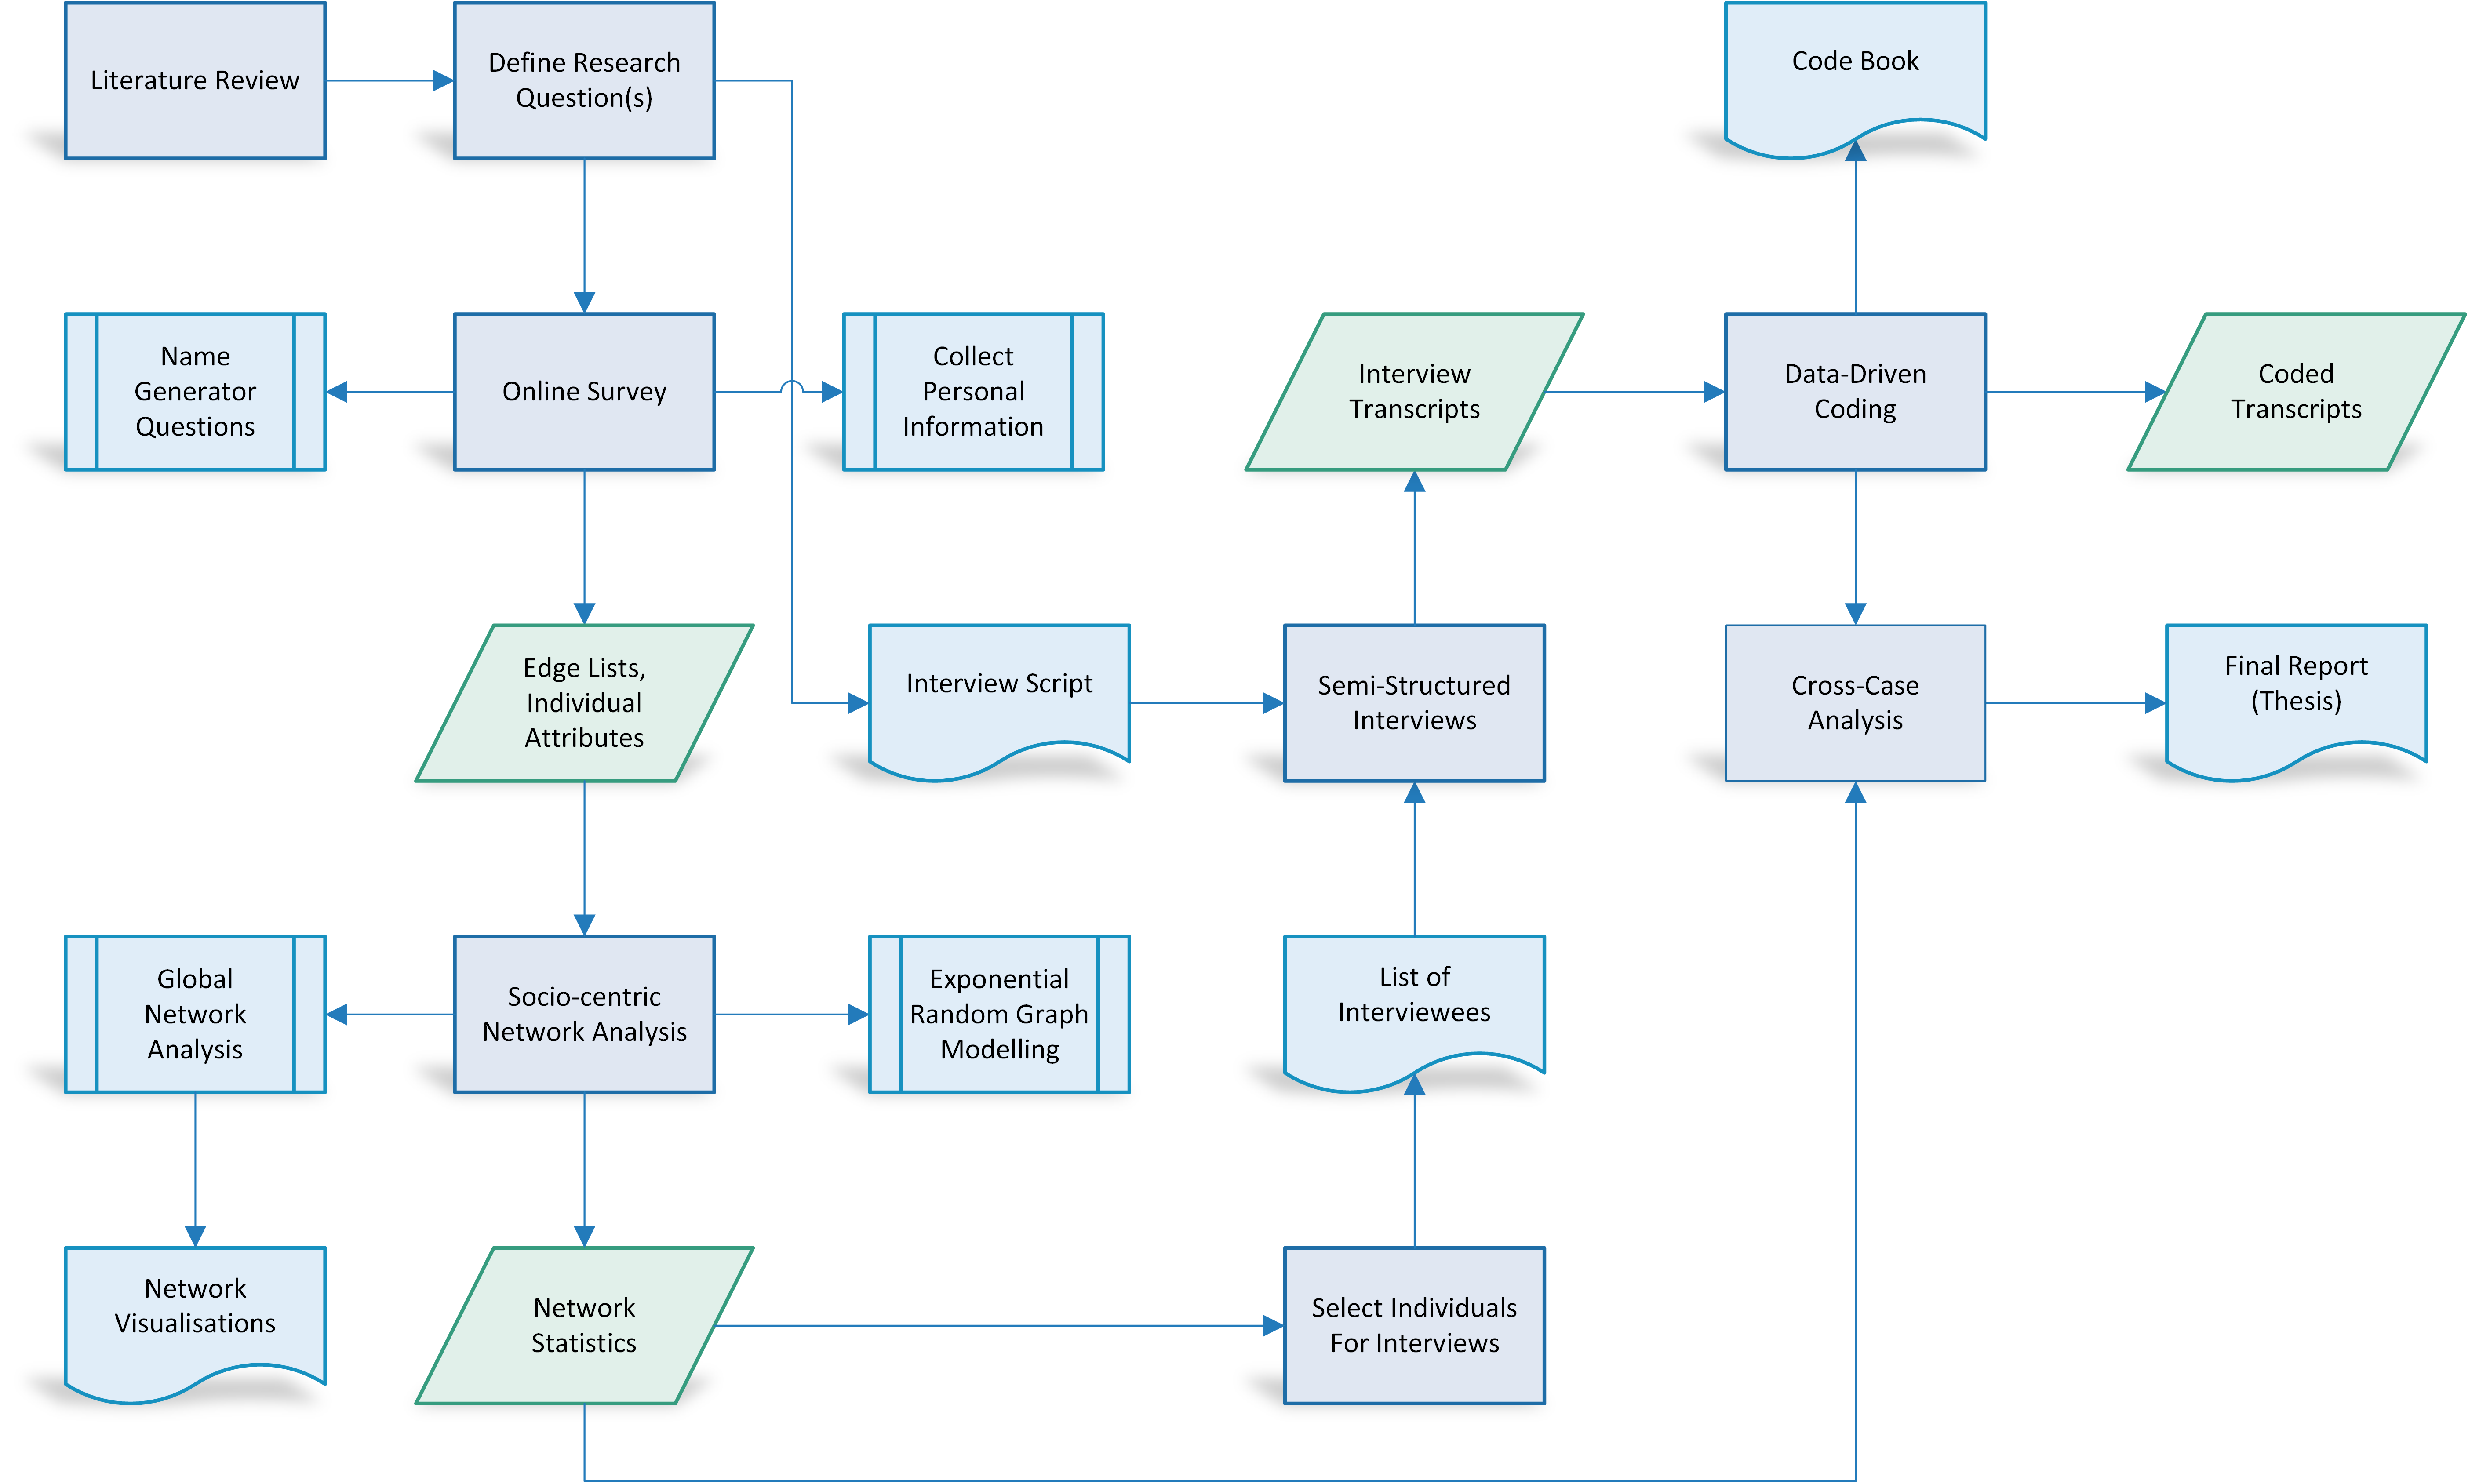
\includegraphics[width=1.0\linewidth]{Images/ResearchPlan_20160909}
		\caption{Mixed methods research design used in this study}
		\label{fig:researchplan20160402}
	\end{figure}
\end{landscape}


\section{Ethics clearance}

Because this study is concerned with human subjects and deals with commercially sensitive information, it had to adhere with the National Statement on Ethical Conduct in Human Research \citep{national2007national}. Data could not be collected without formal ethics approval from both the Commonwealth Scientific and Industrial Research Organisation and Swinburne University of Technology. Approval hinged on individual participants being sufficiently informed to give consent that would allow information about themselves to be used in this study. An application for ethics clearance was submitted to the ethics committees at both organisations. The application included a brief description of this study, a plain language information sheet for participants, a blank consent form, and a list of questions to be included in an on-line survey. Both committees deemed this study low-risk and allowed the collection and subsequent analysis of data to proceed, subject to standard terms and conditions as per the National Statement on Ethical Conduct in Human Research. These include alerting both committees to any changes in data collection procedures and reporting any complaints or issues raised by participants. While some people did decline to participate in this study, none of those who did agree to participate raised any complaints or issues with the way this study was conducted. No changes were made to data collection procedures. \medskip

\section{Research participants}

Finding appropriate candidates for open innovation case studies proved challenging. This study is part of a broader initiative looking at innovation in the food and agriculture sector in a particular region of Australia and cases had to be recruited from this sector. A number of potential candidates were identified using leads provided by agricultural consultants, university researchers, government agencies, and non-governmental organisations. Most firms were not keen on outsiders observing how they went about collaborative innovation. Some firms argued their inter-organisational relationships were a trade-secret and did not want to risk anyone finding out about their strategic intentions. Other firms felt this study would consume too much their time or be too disruptive to their operations. Ultimately, the recruitment of cases relied on a combination of perseverance and goodwill. Despite not having the luxury of choice, the three cases were eventually recruited for this study. \medskip

\begin{table}[]
	\small
	\centering
	\caption{Key characteristics of the cases recruited for this study}
	\label{cases}
	\resizebox{\linewidth}{!}{%
		\begin{tabular}{@{}cllccc@{}}
			\toprule
			Case & \multicolumn{1}{l}{Name}	& \multicolumn{1}{l}{Innovation Challenge}	& Complexity & \begin{tabular}[c]{@{}c@{}}Partner\\ Organisations\end{tabular} & \begin{tabular}[c]{@{}c@{}}Individual\\ Participants\end{tabular} \\ \midrule
			1    & Cold chain innovation		& \begin{tabular}[c]{@{}l@{}}Extend shelf-life of green-leaf\\  vegetables\end{tabular}	& Low		& 7	& 18	\\
			2	& Farm system innovation	& \begin{tabular}[c]{@{}l@{}}Implement robotic dairy system \\ based on voluntary cow traffic\end{tabular}	& High       & 9	& 25	\\
			3	& Collaborative honey bee research	& \begin{tabular}[c]{@{}l@{}}Develop near real-time data analysis \\ system for tracking bee movements\\ in and out of hives\end{tabular} & Mod-High   & 18	& 40 \\ \bottomrule                                                           
		\end{tabular}%
	}
\end{table}

\section{Quantitative procedures}



\subsection{Data collection}

Each case followed the same procedure for collecting and analysing quantitative data. The main contact person in each case was asked to compile a list of people directly involved in the effort. Because this study was aiming for a 100\% participation rate in each case, this person was asked to make sure everybody on their list would be willing to participate in this study. Quantitative data was collected via an on-line survey that captured demographic information about respondents, who they relate to in the collaboration, and how they perceive themselves.\medskip

\subsubsection{Questionnaire design}

The on-line survey needed to be short as an inducement to complete the survey and to avoid responder fatigue \citep{crawford2001web,van2006conducting}. An informal poll amongst workplace colleagues indicated the on-line survey should take no longer than 15 or so minutes to complete. With this limitation in mind, the survey questionnaire was divided into three parts. The first part captured demographic information about the respondent, namely their age, gender, occupation, level and field of education, workplace postcode, relevant work experience, and current job tenure. Response options for categorical questions were based on the Australian and New Zealand Standard Classification of Occupations \citep{pink2009anzsco} and the Australian Standard Classification of Education \citep{trewin2000australian}. Respondents were also asked to state their role in the open innovation collaboration.\medskip

The second part of the questionnaire captured information about specific social relationships. Respondents were asked to name people in the open innovation collaboration they received knowledge and ideas from, felt they could trust, have worked with before, they reported to. Respondents could select names from a drop-down list or add names of people missing from the list. Asking respondents who they receive knowledge and ideas from, rather than who they share knowledge or generate ideas with, was a deliberate move to avoid them nominating everybody in the drop-down list. By asking respondents to nominate who they receive knowledge and ideas from required them to think more carefully about their response. Respondents also had to indicate how much of the knowledge provided to them was tacit in nature. Tacit knowledge may be characterised in terms of complexity, codifiability, and observability \citep{winter987knowledge,zander1995knowledge,cavusgil2003tacit}. Knowledge that is complex, poorly encoded, and mostly acquired through observation is considered to be predominantly tacit in nature. For each knowledge provider, respondents had to rate how complex the knowledge provided to them was, how much of it was documented, and to what extent was it acquired through direct observation on a 10-point scale.\medskip 

The third part of the questionnaire aimed to build a psychological profile of the respondent in terms of personality, self-efficacy, organisational identification, and work motivation. Respondents were presented with a number of statements about themselves, which they had to rate their level of agreement with, using a 10-point scale. Personality was profiled using items from an ultra-shortened version of the Big Five Inventory (BFI-10). This uses two items to measure each of the big five personality traits \citep{rammstedt2007measuring}. Only three personality traits positively correlated with knowledge sharing were profiled: agreeableness, conscientiousness, and openness to experience \citep{matzler2008personality,matzler2011personality}. While the BFI-10 is a less reliable scale (agreeableness: $\alpha$ = 0.42, conscientiousness: $\alpha$ = 0.67, emotional stability: $\alpha$ = 0.78, extraversion: $\alpha$ = 0.79, openness: $\alpha$ = 0.50), it is sufficient for research settings with tight time-constraints \citep{rammstedt2007measuring}.\medskip

Self-efficacy was assessed in terms of how competent one felt doing one's job, sense of self-determination, and confidence in one's ability to come up with creative ideas or solutions. Job competence and self-determination was profiled using statements from the Measuring Empowerment Scale \citep{spreitzer1995psychological}. Internal reliability of this scale is considered good (job competence: $\alpha$ = 0.81, self-determination: $\alpha$ = 0.81). The ability to come up with creative ideas or solutions was profiled using statements from the Creative Self-Efficacy Scale \citep{tierney2002creative}. Past studies indicate this scale is reliable with reported $\alpha$ values between 0.74 and 0.91 \citep{tierney2002creative,gong2009employee,tierney2011creative,mittal2015transformational}.\medskip

The Organisational Identification Scale \citep{mael1992alumni} was used to assess how strongly the respondent identified with his or her work-group, employer, and with the collaboration more broadly. This scale has proved to be reliable in a variety of study settings with reported $\alpha$ values between 0.73 and 0.89 \citep{mael1992alumni,bergami2000self,knippenberg2000foci,van2008interactive}. Only one of the six items in the scale was used in this survey: "when someone criticises my organisation, it feels like an insult". It has the highest factor loading of all six items \citep{mael1992identifying} and was adapted to address identification with one's work-group, with one's employer, and with the collaboration more broadly. Using all six items for each of these cases would of been impractical, given the time constraint in which to complete the survey.\medskip

Work motivation was measured using the 19-item Multidimensional Work Motivation Scale \citep{gagne2015multidimensional}. Tested in various cultural and language contexts, this scale has sub-scales for amotivation, extrinsic material regulation, extrinsic social regulation, introjected regulation, identified regulation, and intrinsic motivation. Reliability of the English version is good with reported $\alpha$ values between 0.79 and 0.90. Items in the Multidimensional Work Motivation Scale were modified to suit the study context. For example, the scale has a stem question: “Why do you or would you put efforts into your current job”? One response option is: "Because I personally consider it important to put efforts in this job". This was modified to read as thus: "I put effort into this collaboration because I personally consider it important to do so". \medskip

\subsubsection{Piloting of the survey}

For quality assurance, the on-line survey was piloted twice to check (a) if questions were clear and not ambiguous, and (b) how long it would take to complete on-line survey. Ten people were involved in each pilot. Apart from one question about trust, everybody in the first pilot reported no issues with clarity or ambiguity. One person felt the question asking respondents to name people in the collaboration they trust needed to be reworded. This person thought the question was asking respondents to pass judgement on others. This suggestion was taken on board and the question changed accordingly. Everybody involved in the second pilot was comfortable with the survey though one person felt the invitation email was too long. Most of the people in each pilot completed the survey within 20 minutes. The only exceptions were people who took their time making detailed notes as they went through the survey. Table \ref{tab:self-report} lists the 59 items used in the on-line survey, together with associated response options and references.\medskip  


\subsubsection{Survey procedure}

The aforementioned list of people involved in the open innovation collaboration also included their email addresses. People on the list were sent an email message inviting them to complete the web-based survey questionnaire. The email message provided information about the study and included a unique link to the survey website\footnote{the web-based survey was hosted by ONASurveys, a company specialising in social network surveys (http://www.onasurveys.com).}. People could either ignore the email invitation or agree to take part in the survey by clicking on the URL link provided. Those who clicked on the link were directed to the survey website where they were first asked to give consent for their survey responses to be used in this study before being able to complete the on-line survey.\medskip



 

% survey


\section{Network measures}

Eigenvector centrality considers node importance. A node is considered important if it is linked to other important nodes. Eigenvector centrality differs from in-degree centrality: a node receiving many links does not necessarily have a high eigenvector centrality (it might be that all linkers have low or null eigenvector centrality). Moreover, a node with high eigenvector centrality is not necessarily highly linked (the node might have few but important linkers). 

\subsection{Data analysis}

\begin{table}[]
	\tiny
	\centering
	\caption{Exponential random graph model parameters used in this study.}
	\label{erm_params}
	\begin{tabular}{lcl}
		\toprule
		Parameter & Graphic & Explanation  \\ \midrule
		\textbf{Purely structural effects} & & \\
		Arc (edge)                    	& \begin{minipage}{.2\textwidth} \centering 
\includegraphics[width=0.4\linewidth]{Images/Arc} \end{minipage} 					& \begin{tabular}[c]{l}Baseline propensity for a tie to form in the absence of other\\ effects.\end{tabular} \\ \\
		Reciprocity (mutuality)       	& \begin{minipage}{.2\textwidth} \centering 
\includegraphics[width=0.4\linewidth]{Images/Reciprocity} \end{minipage} 			& \begin{tabular}[c]{l}Propensity for a tie from one actor to a second when there\\ is already a tie from the second to the first.\end{tabular} \\ \\                                                                                                       \\
		TwoPath (simple connectivity) 	& \begin{minipage}{.2\textwidth} \centering \includegraphics[width=0.4\linewidth]{Images/Twopath} \end{minipage}        		& \begin{tabular}[c]{l}Propensity for ties to form as part of simple path formations. \end{tabular} \\ \\
		AinS (popularity spread)      	& \begin{minipage}{.2\textwidth} \centering 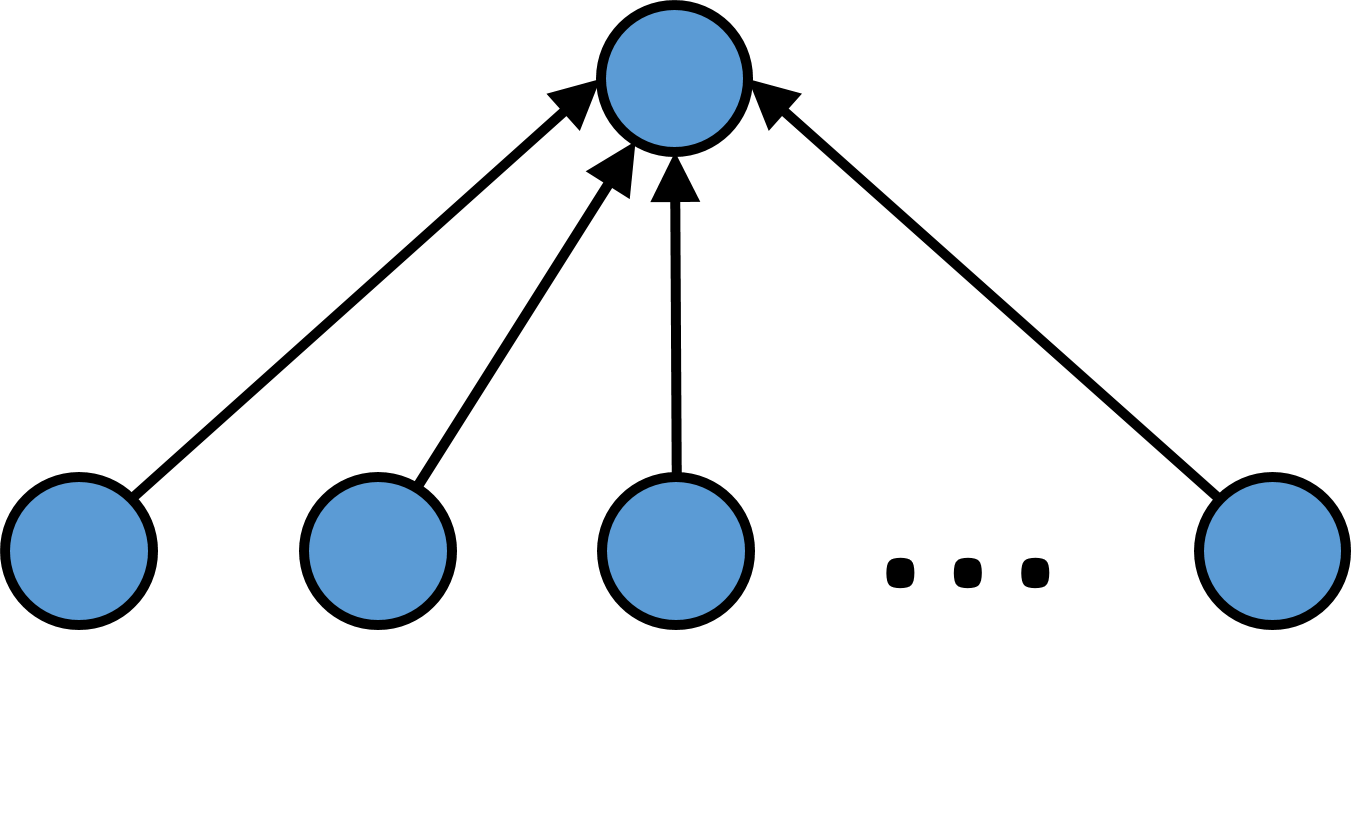
\includegraphics[width=0.6\linewidth]{Images/AinS} \end{minipage}        			& \begin{tabular}[c]{l}Propensity for dispersion in the in-degree distribution,\\ indicating there are a few highly popular actors. \end{tabular} \\ \\
		AoutS (activity spread)       	& \begin{minipage}{.2\textwidth} \centering 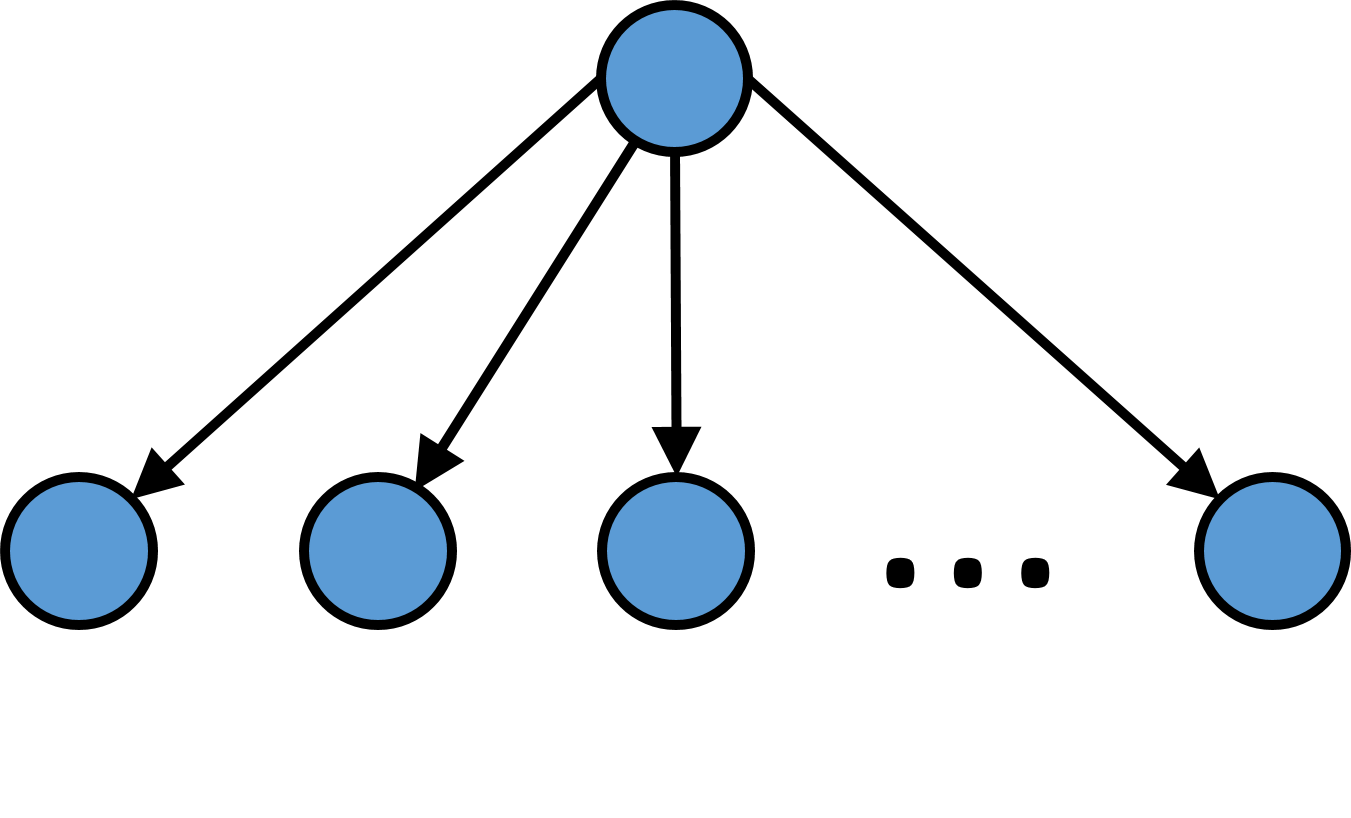
\includegraphics[width=0.6\linewidth]{Images/AoutS} \end{minipage}  				& \begin{tabular}[c]{l}Propensity for dispersion in the out-degree distribution,\\ indicating there are a few highly active actors. \end{tabular}  \\ \\
		AT-T (path closure)           	& \begin{minipage}{.2\textwidth} \centering 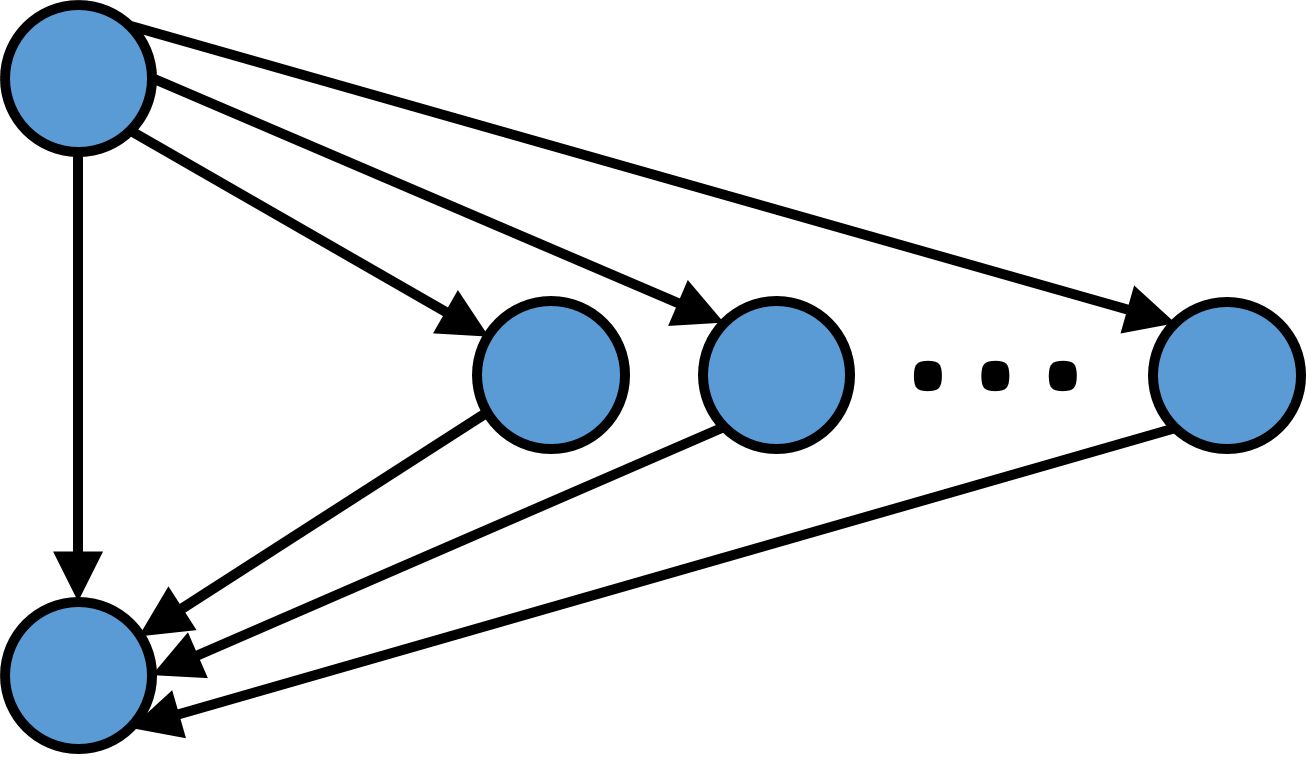
\includegraphics[width=0.6\linewidth]{Images/AT-T} \end{minipage}        			& \begin{tabular}[c]{l}Propensity for ties to form as part of transitive triad or a\\ multiple transitive configuration. \end{tabular} \\ \\
		AT-C (cyclic closure)         	& \begin{minipage}{.2\textwidth} \centering 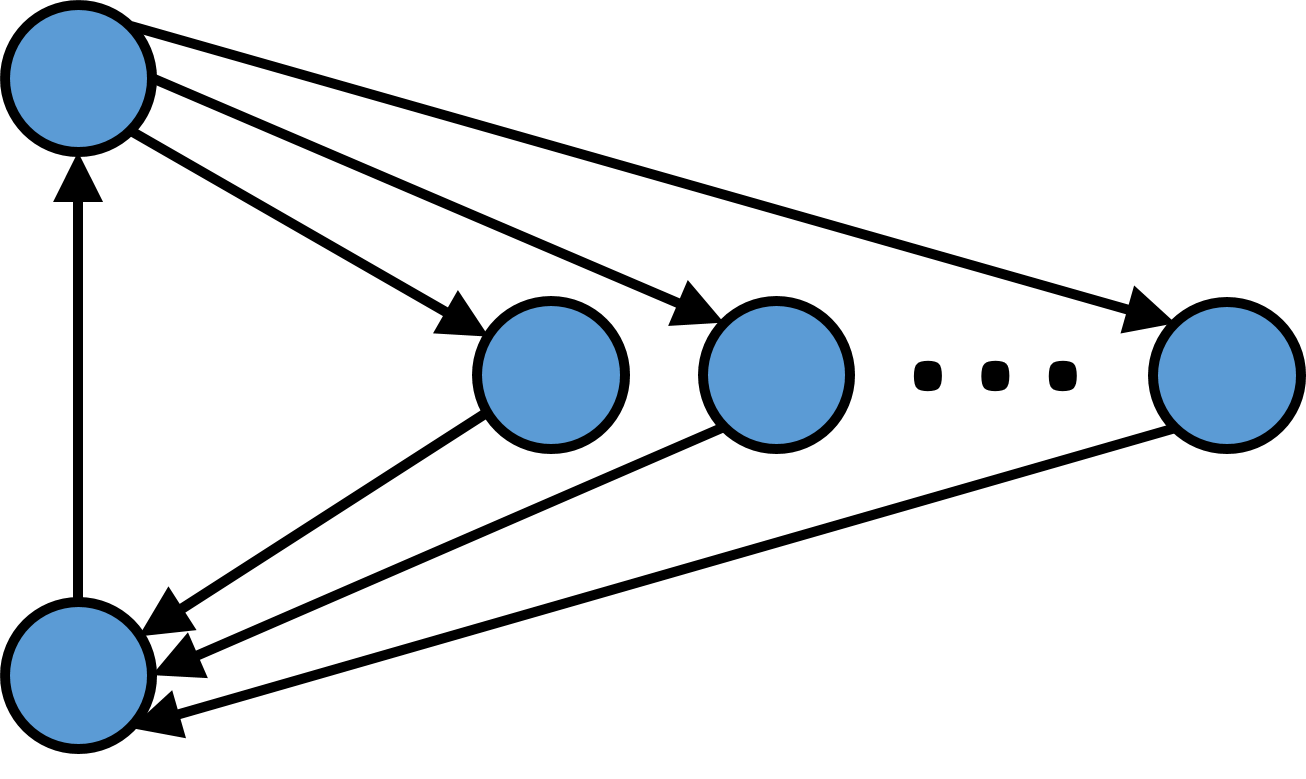
\includegraphics[width=0.6\linewidth]{Images/AT-C} \end{minipage}        			& \begin{tabular}[c]{l}Propensity for ties to form as part of a cyclic triad or a\\ multiple cyclic configuration. \end{tabular} \\ \\
		A2P (multiple connectivity)   	& \begin{minipage}{.2\textwidth} \centering 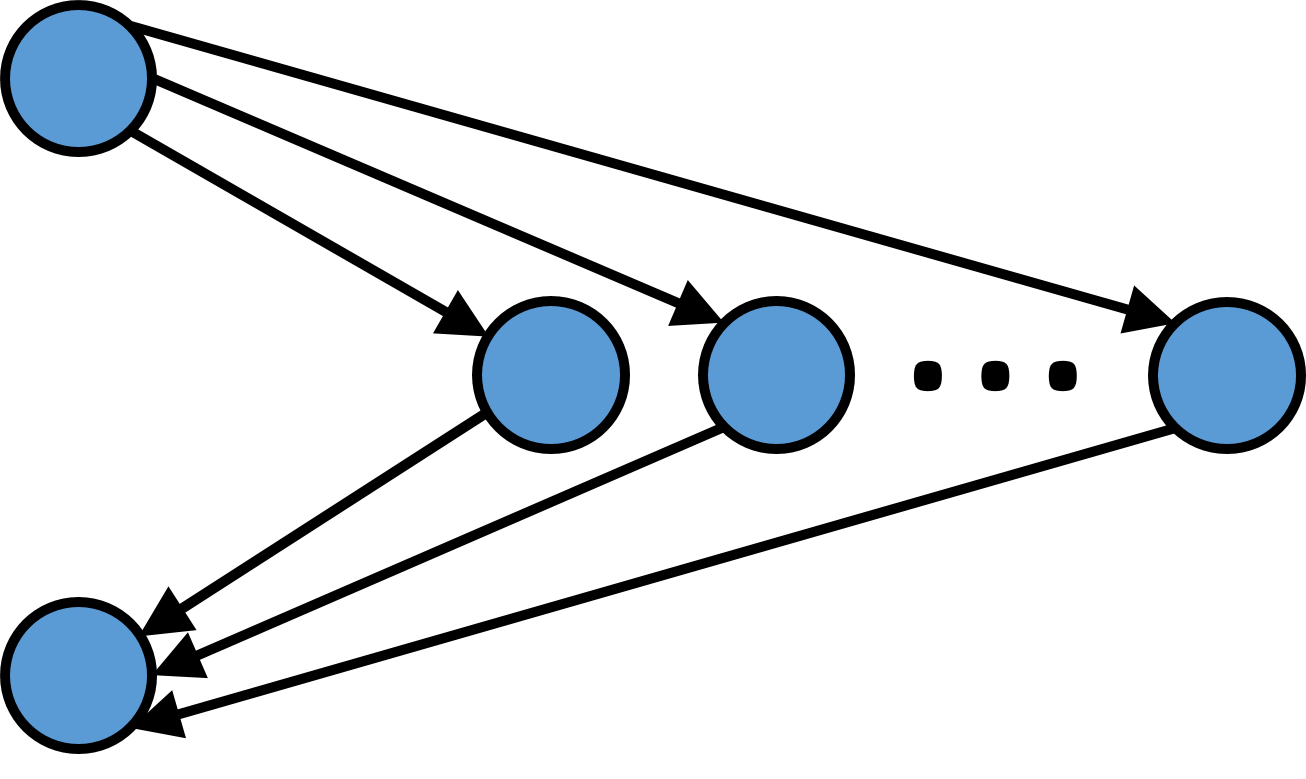
\includegraphics[width=0.6\linewidth]{Images/A2P} \end{minipage}       				& \begin{tabular}[c]{l}Propensity for ties to form as part of formations involving\\ multiple short paths between actors. \end{tabular} \\ \\
		\textbf{Actor-relation effects} & & \\
		Attribute sender              	& \begin{minipage}{.2\textwidth} \centering 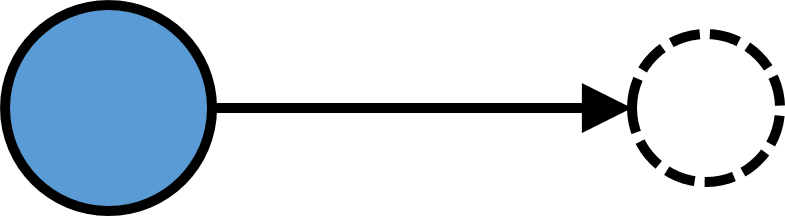
\includegraphics[width=0.4\linewidth]{Images/Sender} \end{minipage}        			& \begin{tabular}[c]{l}Propensity for a tie to be directed from an actor with a\\ particular attribute. \end{tabular} \\ \\
		Attribute receiver             	& \begin{minipage}{.2\textwidth} \centering 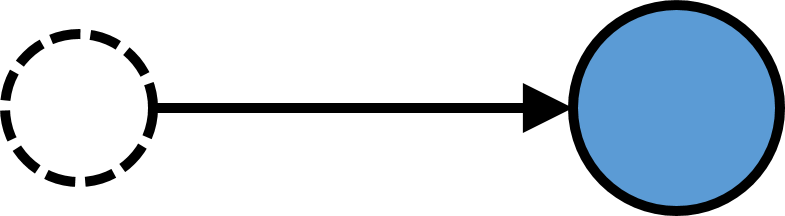
\includegraphics[width=0.4\linewidth]{Images/Receiver} \end{minipage}        		& \begin{tabular}[c]{l}Propensity for a tie to be directed toward an actor with a\\ particular attribute. \end{tabular} \\ \\
		Attribute match               	& \begin{minipage}{.2\textwidth} \centering 
\includegraphics[width=0.4\linewidth]{Images/Match} \end{minipage}       			& \begin{tabular}[c]{l}Propensity for a tie to form between actors with the same\\ categorical attribute.\end{tabular} \\ \\
		Attribute mismatch reciprocity 	& \begin{minipage}{.2\textwidth} \centering 
\includegraphics[width=0.4\linewidth]{Images/MisMatchReciprocity} \end{minipage}  	& \begin{tabular}[c]{l}Propensity for a tie to form between actors with a\\ non-matching categorical attribute.\end{tabular} \\ \\
		Attribute difference          	& \begin{minipage}{.2\textwidth} \centering 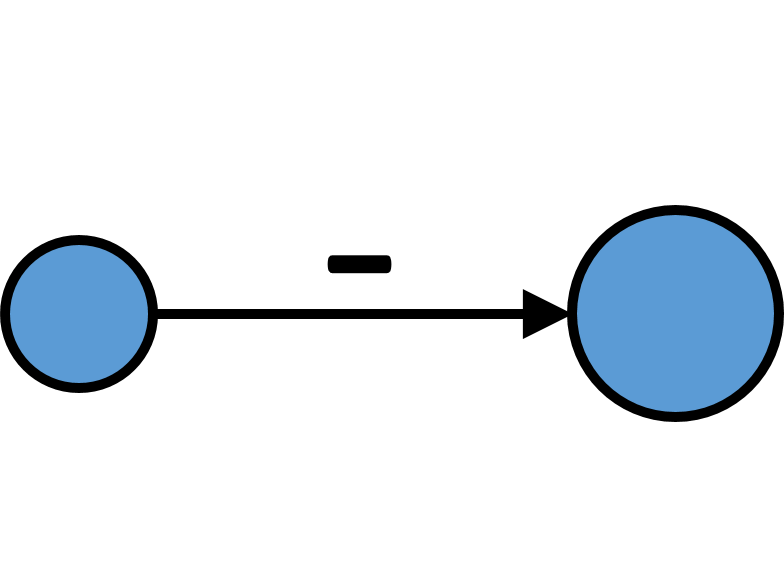
\includegraphics[width=0.4\linewidth]{Images/Difference} \end{minipage}       		& \begin{tabular}[c]{l}Propensity for a tie to form between actors with a similar\\ continuous attribute. \end{tabular} \\ \\
		Attribute product             	& \begin{minipage}{.2\textwidth} \centering 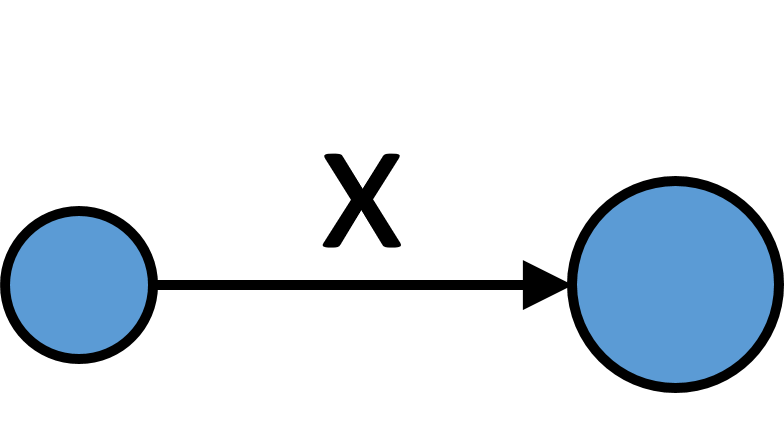
\includegraphics[width=0.4\linewidth]{Images/Product} \end{minipage}        		& \begin{tabular}[c]{l}Propensity for a tie to form between actors who both score\\ highly on the same continuous attribute. \end{tabular} \\ \\
		\textbf{Actor-brokerage effects} & & \\
		b\textsubscript{O} (liaison role)			      	&  \begin{minipage}{.2\textwidth} \centering 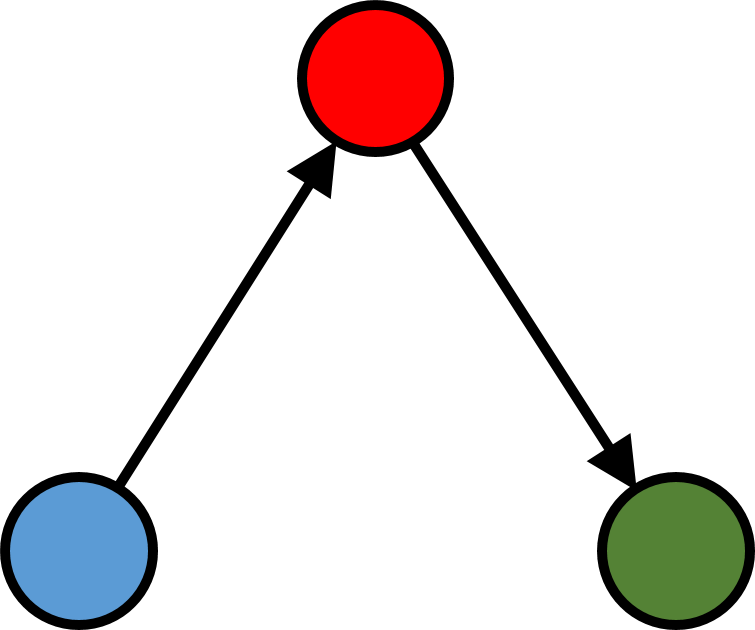
\includegraphics[width=0.4\linewidth]{Images/b_O} \end{minipage}   & \begin{tabular}[c]{l}Propensity to have brokers who mediate communication\\ between two individuals from different groups, neither of\\ which they belong to.\end{tabular}\\ \\
		b\textsubscript{IO} (representative role)		   	& \begin{minipage}{.2\textwidth} \centering 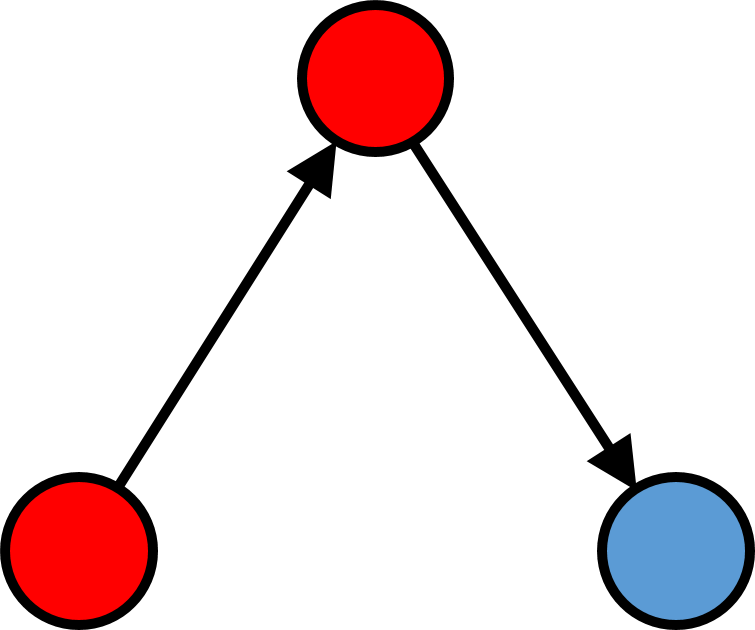
\includegraphics[width=0.4\linewidth]{Images/b_IO} \end{minipage}   & \begin{tabular}[c]{l}Propensity to have brokers who mediate communication\\ from in-group members to out-group members.\end{tabular}\\ \\
		b\textsubscript{OI} (gatekeeper role) 				& \begin{minipage}{.2\textwidth} \centering 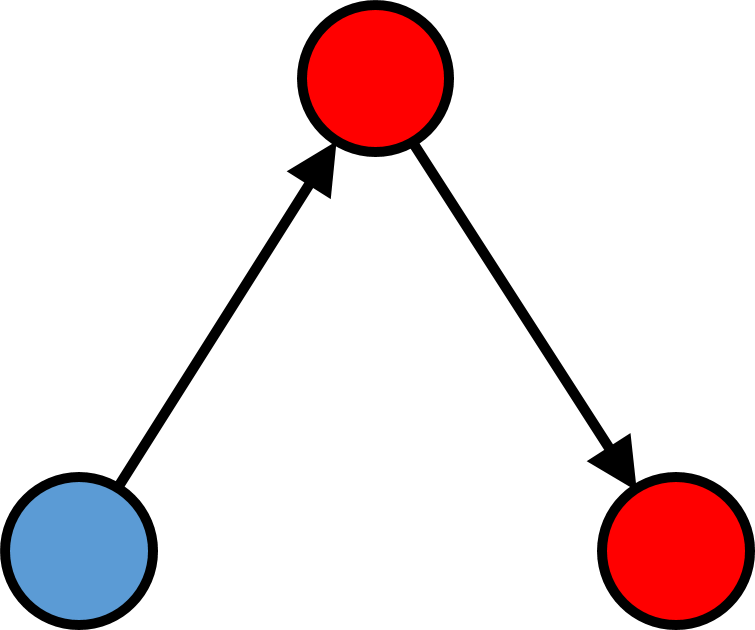
\includegraphics[width=0.4\linewidth]{Images/b_OI} \end{minipage}   & \begin{tabular}[c]{l}Propensity to have brokers who mediate communication\\ from out-group members to in-group members. \end{tabular}\\ \\
		w{\textsubscript{O} (itinerant broker)			&  \begin{minipage}{.2\textwidth} \centering 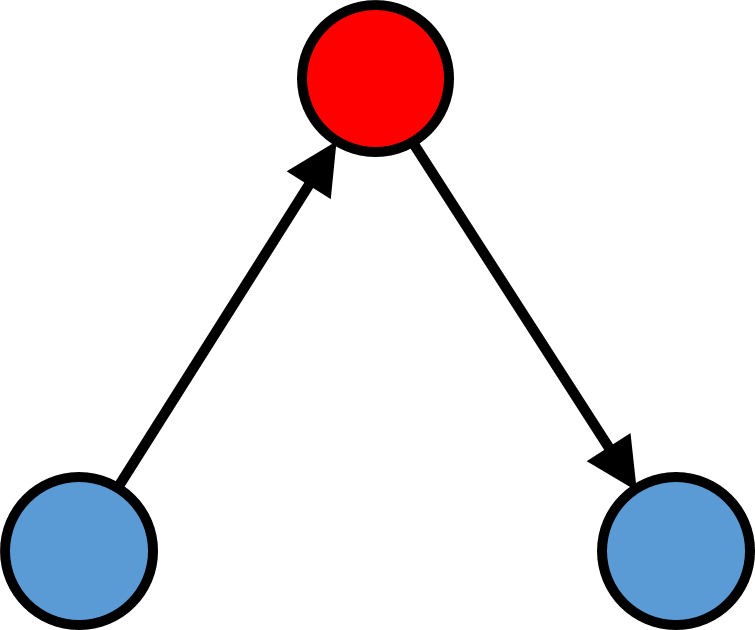
\includegraphics[width=0.4\linewidth]{Images/w_O} \end{minipage}   & \begin{tabular}[c]{l}Propensity to have brokers who mediate communication\\ between two individuals from a single group to which they\\ do not belong. \end{tabular}\\ 
		w\textsubscript{I} (coordination role)				& \begin{minipage}{.2\textwidth} \centering 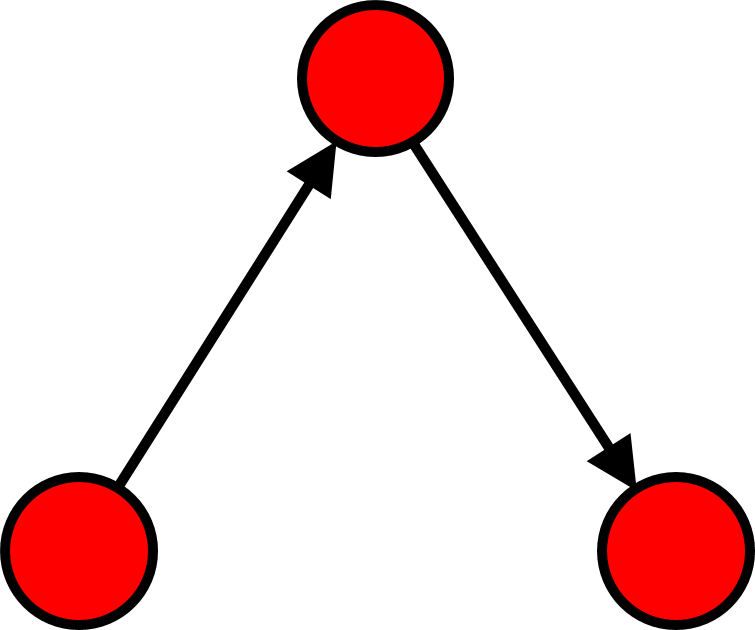
\includegraphics[width=0.4\linewidth]{Images/w_I} \end{minipage}    & \begin{tabular}[c]{l}Propensity to have brokers who mediate communication\\ between two individuals from his or her own group. \end{tabular}\\ \\	
		\textbf{Network covariate effects} & & \\
		Dyadic covariate             	& \begin{minipage}{.2\textwidth} \centering 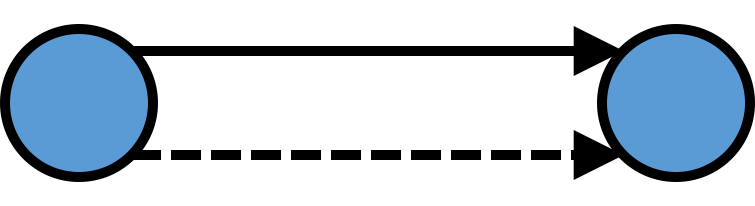
\includegraphics[width=0.4\linewidth]{Images/DyadicCovariate} \end{minipage}    	& \begin{tabular}[c]{l}Propensity for a tie of one type to form from one actor to\\ another if a tie of another type is already present, though\\ the covariate network is fixed (i.e. exogenous) in the\\ model, and so cannot vary. \end{tabular} \\\bottomrule                                                                                                       
	\end{tabular}
\end{table}